\chapter{\label{ch:8-appendix}Appendices} 

\graphicspath{{figures/appendix/}}

\begin{figure}[h]
	\centering
	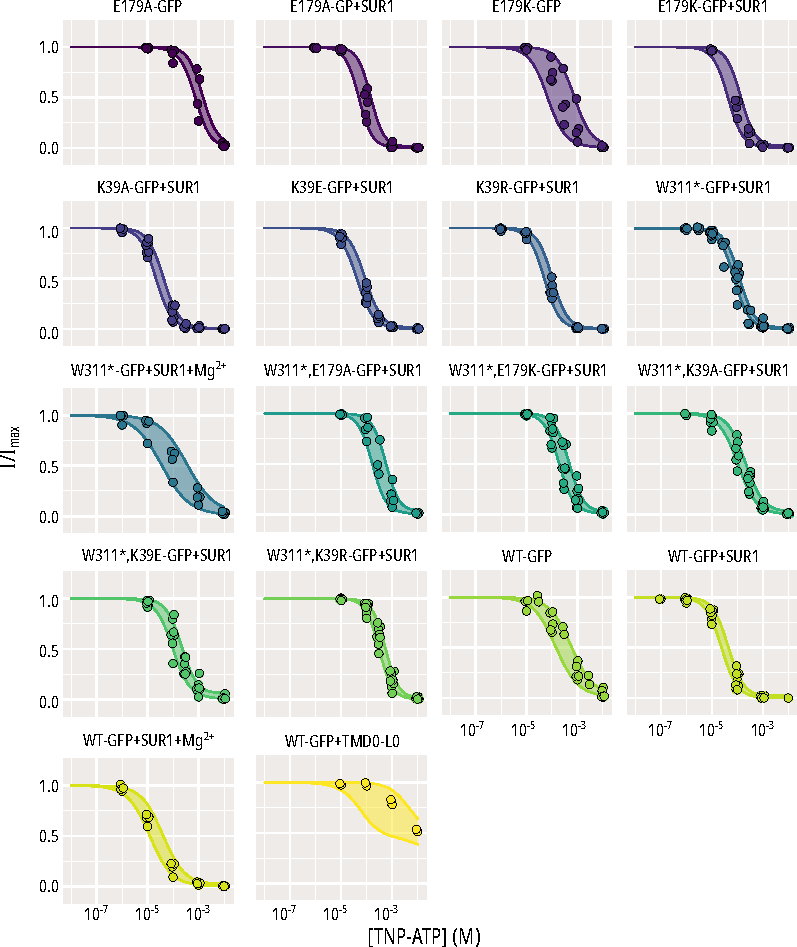
\includegraphics[width=\textwidth]{all_atp_fits.pdf}
	\caption[ATP inhibition population hill fits]{
	Inhibition of current by ATP in excised patches expressing each of the constructs and conditions tested in this thesis.
	Each point represents an individual measurement normalised to the average of the current measured immediately before ATP perfusion, and immediately after ATP washout.
	The smooth filled curves are the \SI{95}{\percent} intervals of the posterior probability distribution of fits to equation \ref{eq:hill} as described in the methods, marginalising over the \textgreek{d}\textsubscript{experiment}.
	}
	\label{apxfig:atp_inhib_1}
\end{figure}

\begin{figure}[h]
	\centering
	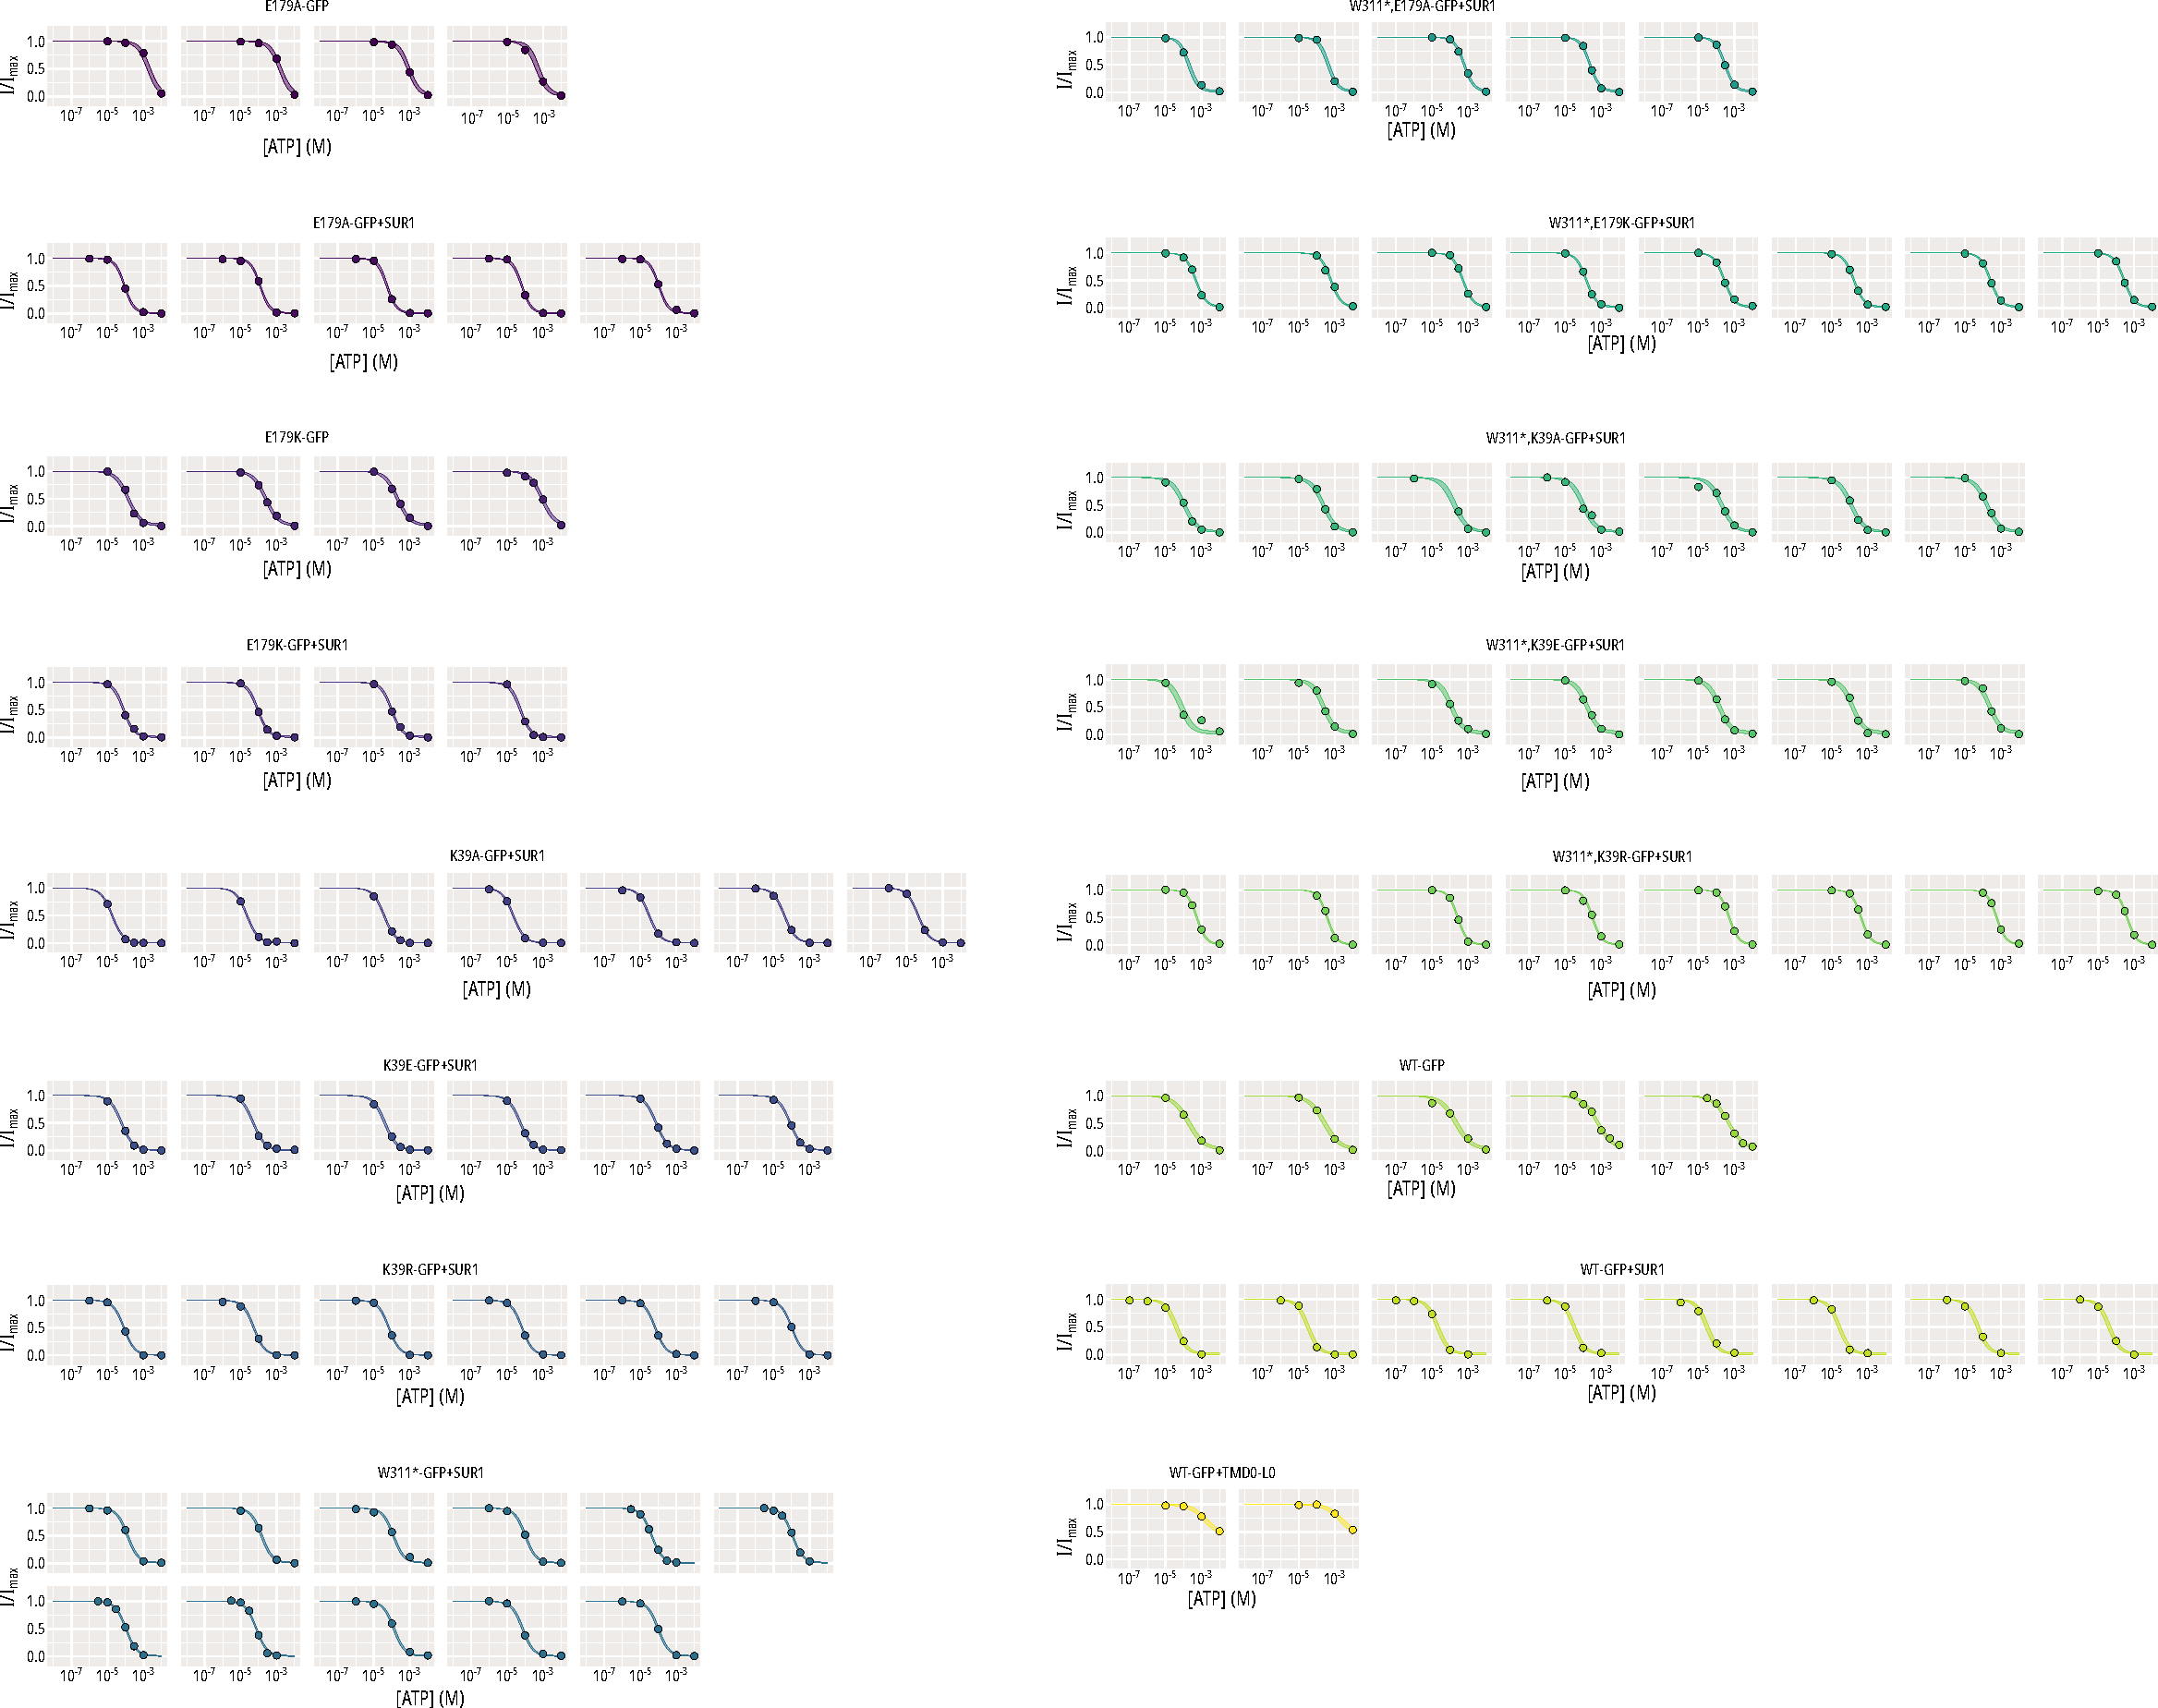
\includegraphics[width=\textwidth]{all_atp_fits_2.pdf}
	\caption[ATP inhibition sample hill fits]{
	Inhibition of current by ATP in excised patches expressing each of the constructs and conditions tested in this thesis, with each individual experiment plotted separately.
	Each point represents an individual measurement normalised to the average of the current measured immediately before ATP perfusion, and immediately after ATP washout.
	The smooth filled curves are the \SI{95}{\percent} intervals of the posterior probability distribution of fits to equation \ref{eq:hill} as described in the methods, including the \textgreek{d}\textsubscript{experiment}.
	}
	\label{apxfig:atp_inhib_2}
\end{figure}

\begin{figure}[h]
	\centering
	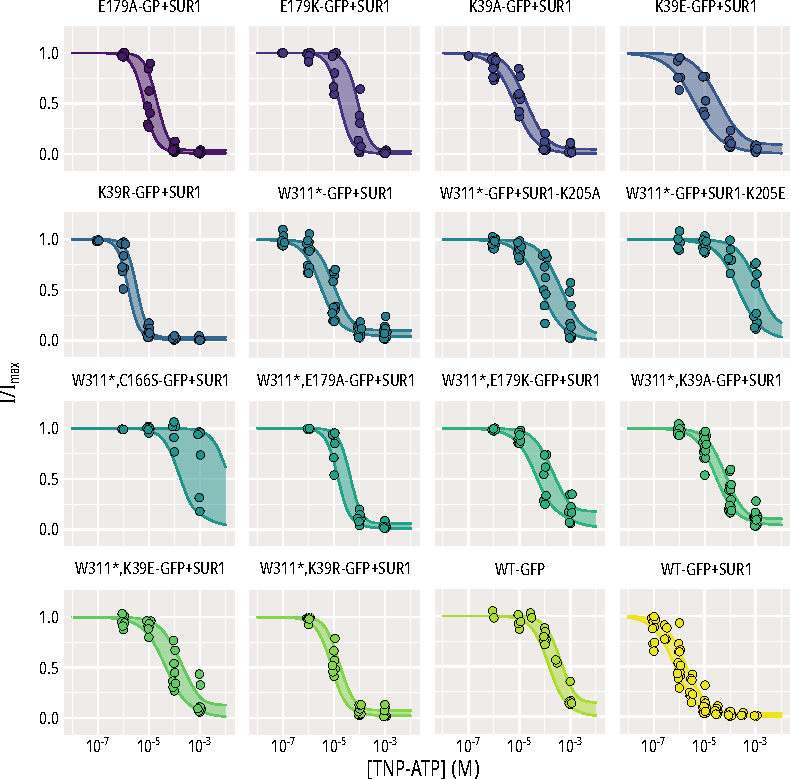
\includegraphics[width=\textwidth]{all_tnpatp_fits.pdf}
	\caption[TNP-ATP inhibition population hill fits]{
	Inhibition of current by TNP-ATP in excised patches expressing each of the constructs and conditions tested in this thesis.
	Each point represents an individual measurement normalised to the average of the current measured immediately before TNP-ATP perfusion, and immediately after TNP-ATP washout.
	The smooth filled curves are the \SI{95}{\percent} intervals of the posterior probability distribution of fits to equation \ref{eq:hill} as described in the methods, marginalising over the \textgreek{d}\textsubscript{experiment}.
	}
	\label{apxfig:tnpatp_inhib_1}
\end{figure}

\begin{figure}[h]
	\centering
	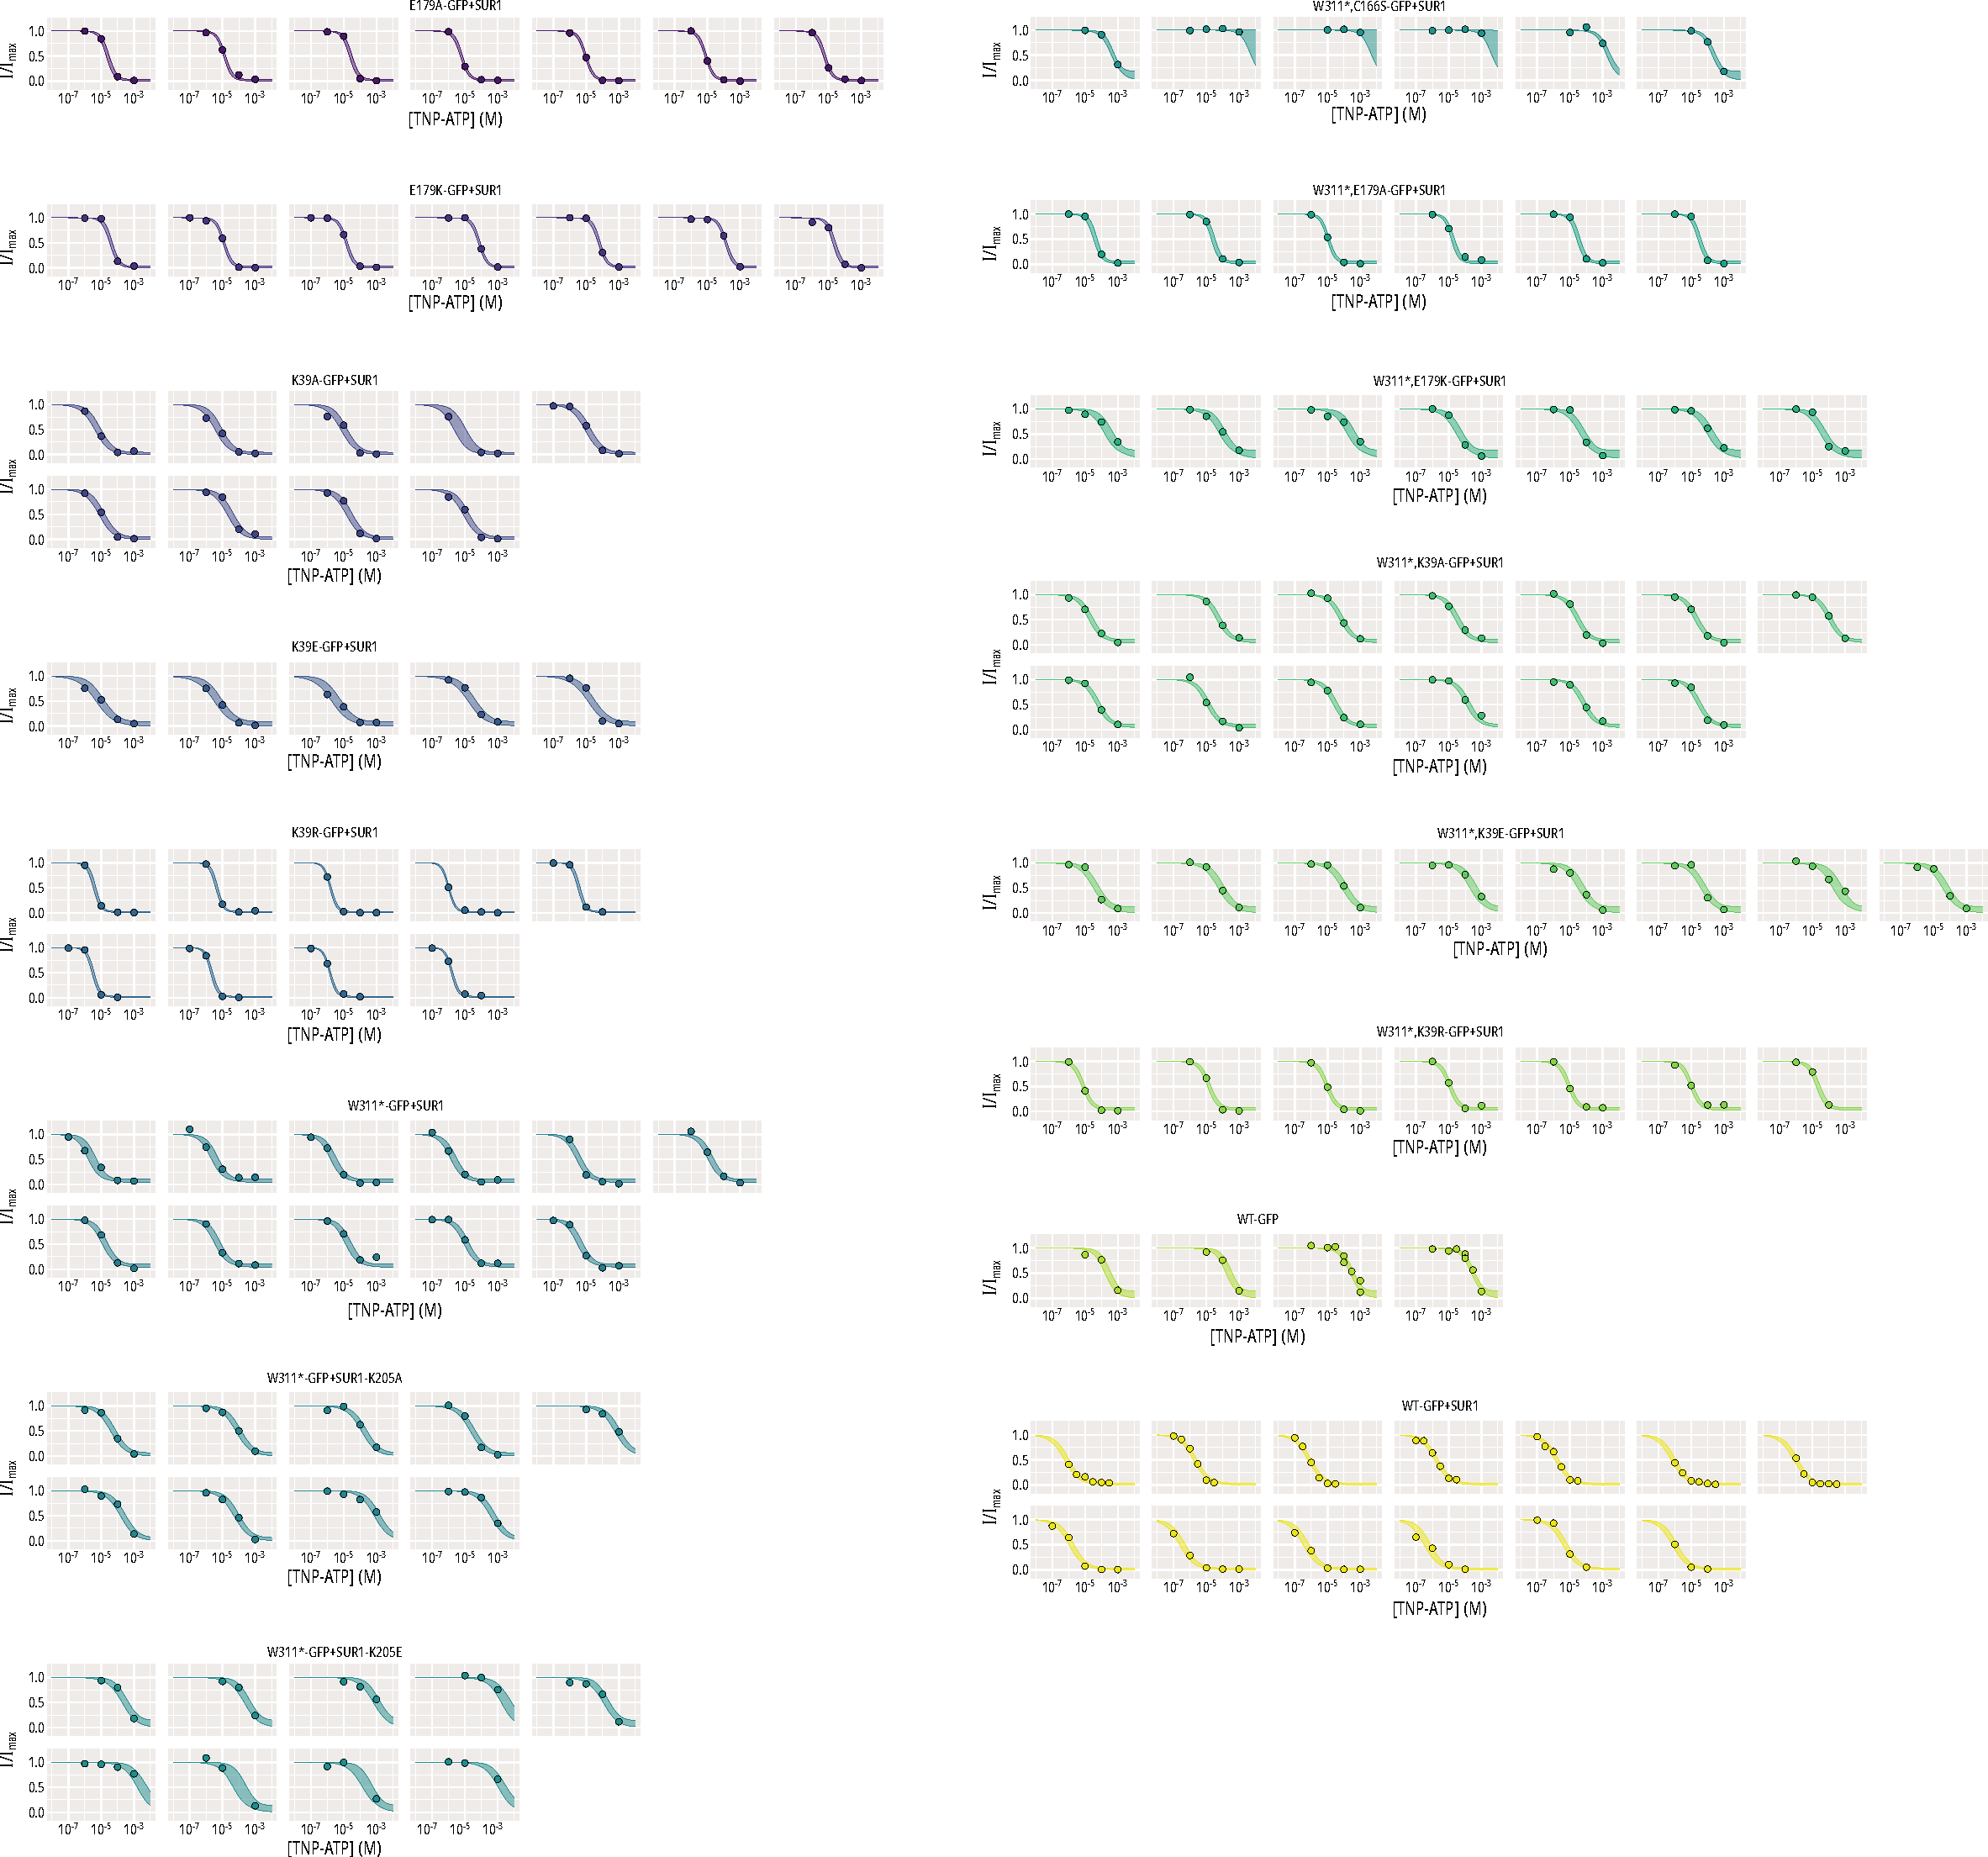
\includegraphics[width=\textwidth]{all_tnpatp_fits_2.pdf}
	\caption[TNP-ATP inhibition sample hill fits]{
	Inhibition of current by TNP-ATP in excised patches expressing each of the constructs and conditions tested in this thesis, with each individual experiment plotted separately.
	Each point represents an individual measurement normalised to the average of the current measured immediately before TNP-ATP perfusion, and immediately after TNP-ATP washout.
	The smooth filled curves are the \SI{95}{\percent} intervals of the posterior probability distribution of fits to equation \ref{eq:hill} as described in the methods, including the \textgreek{d}\textsubscript{experiment}.
	}
	\label{apxfig:tnpatp_inhib_2}
\end{figure}

\begin{figure}[h]
	\centering
	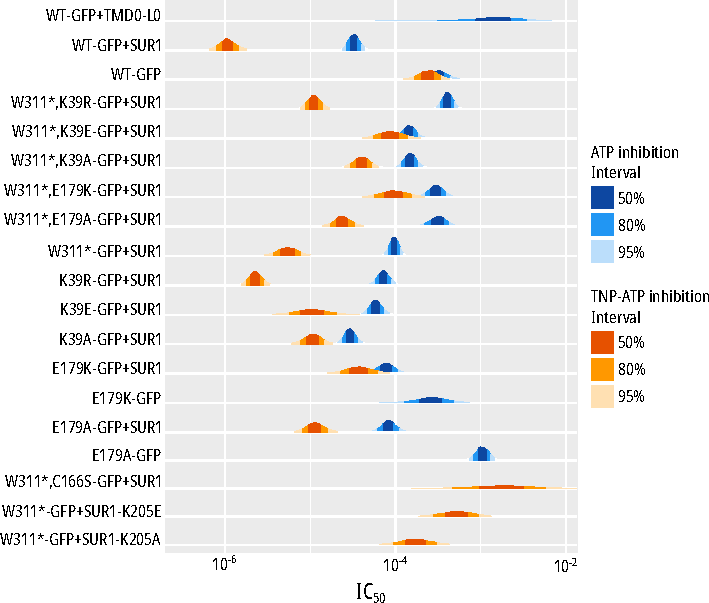
\includegraphics[width=\textwidth]{all_inhibition_params.pdf}
	\caption[Nucleotide inhibition IC\textsubscript{50} posterior distributions]{
	Posterior probability distributions for the population $IC_{50}$ values for inhibition by ATP (blue) or TNP-ATP (orange) from the fits in Figures \ref{apxfig:atp_inhib_1} and \ref{apxfig:tnpatp_inhib_1}
	}
	\label{apxfig:inhib_params}
\end{figure}

\begin{figure}[h]
	\centering
	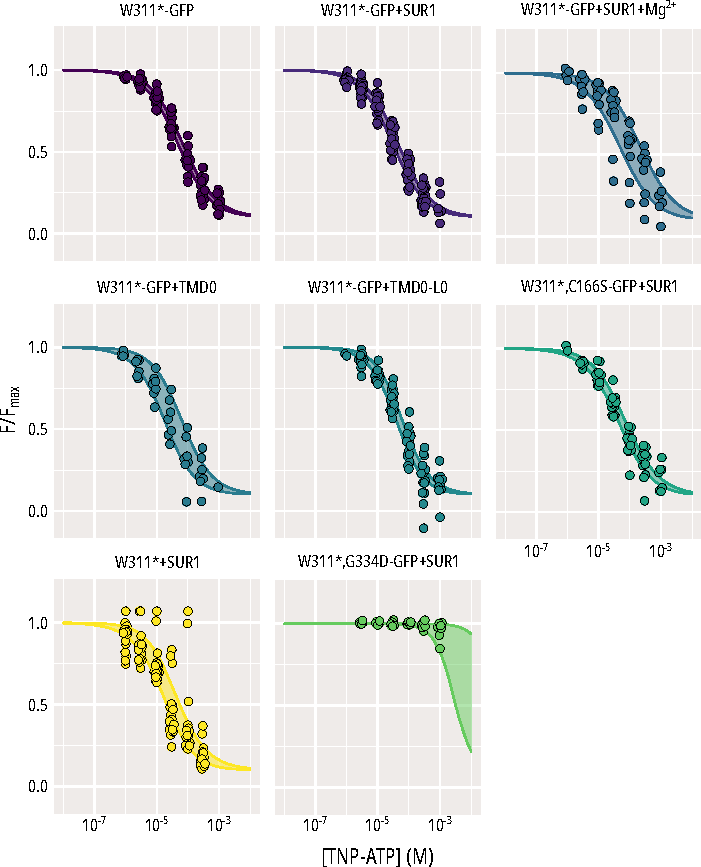
\includegraphics[width=\textwidth]{all_unroofed_fits_1.pdf}
	\caption[Unroofed membrane quenching population hill fits]{
	Quenching of ANAP fluorescence by TNP-ATP in unroofed membrane patches expressing each of the constructs and conditions tested in this thesis.
	Each point represents an individual measurement normalised to the average of the current measured immediately before TNP-ATP perfusion, and immediately after TNP-ATP washout.
	The smooth filled curves are the \SI{95}{\percent} intervals of the posterior probability distribution of fits to equation \ref{eq:hill} as described in the methods, marginalising over the \textgreek{d}\textsubscript{experiment}.
	}
	\label{apxfig:unroofed_1}
\end{figure}

\begin{figure}[h]
	\centering
	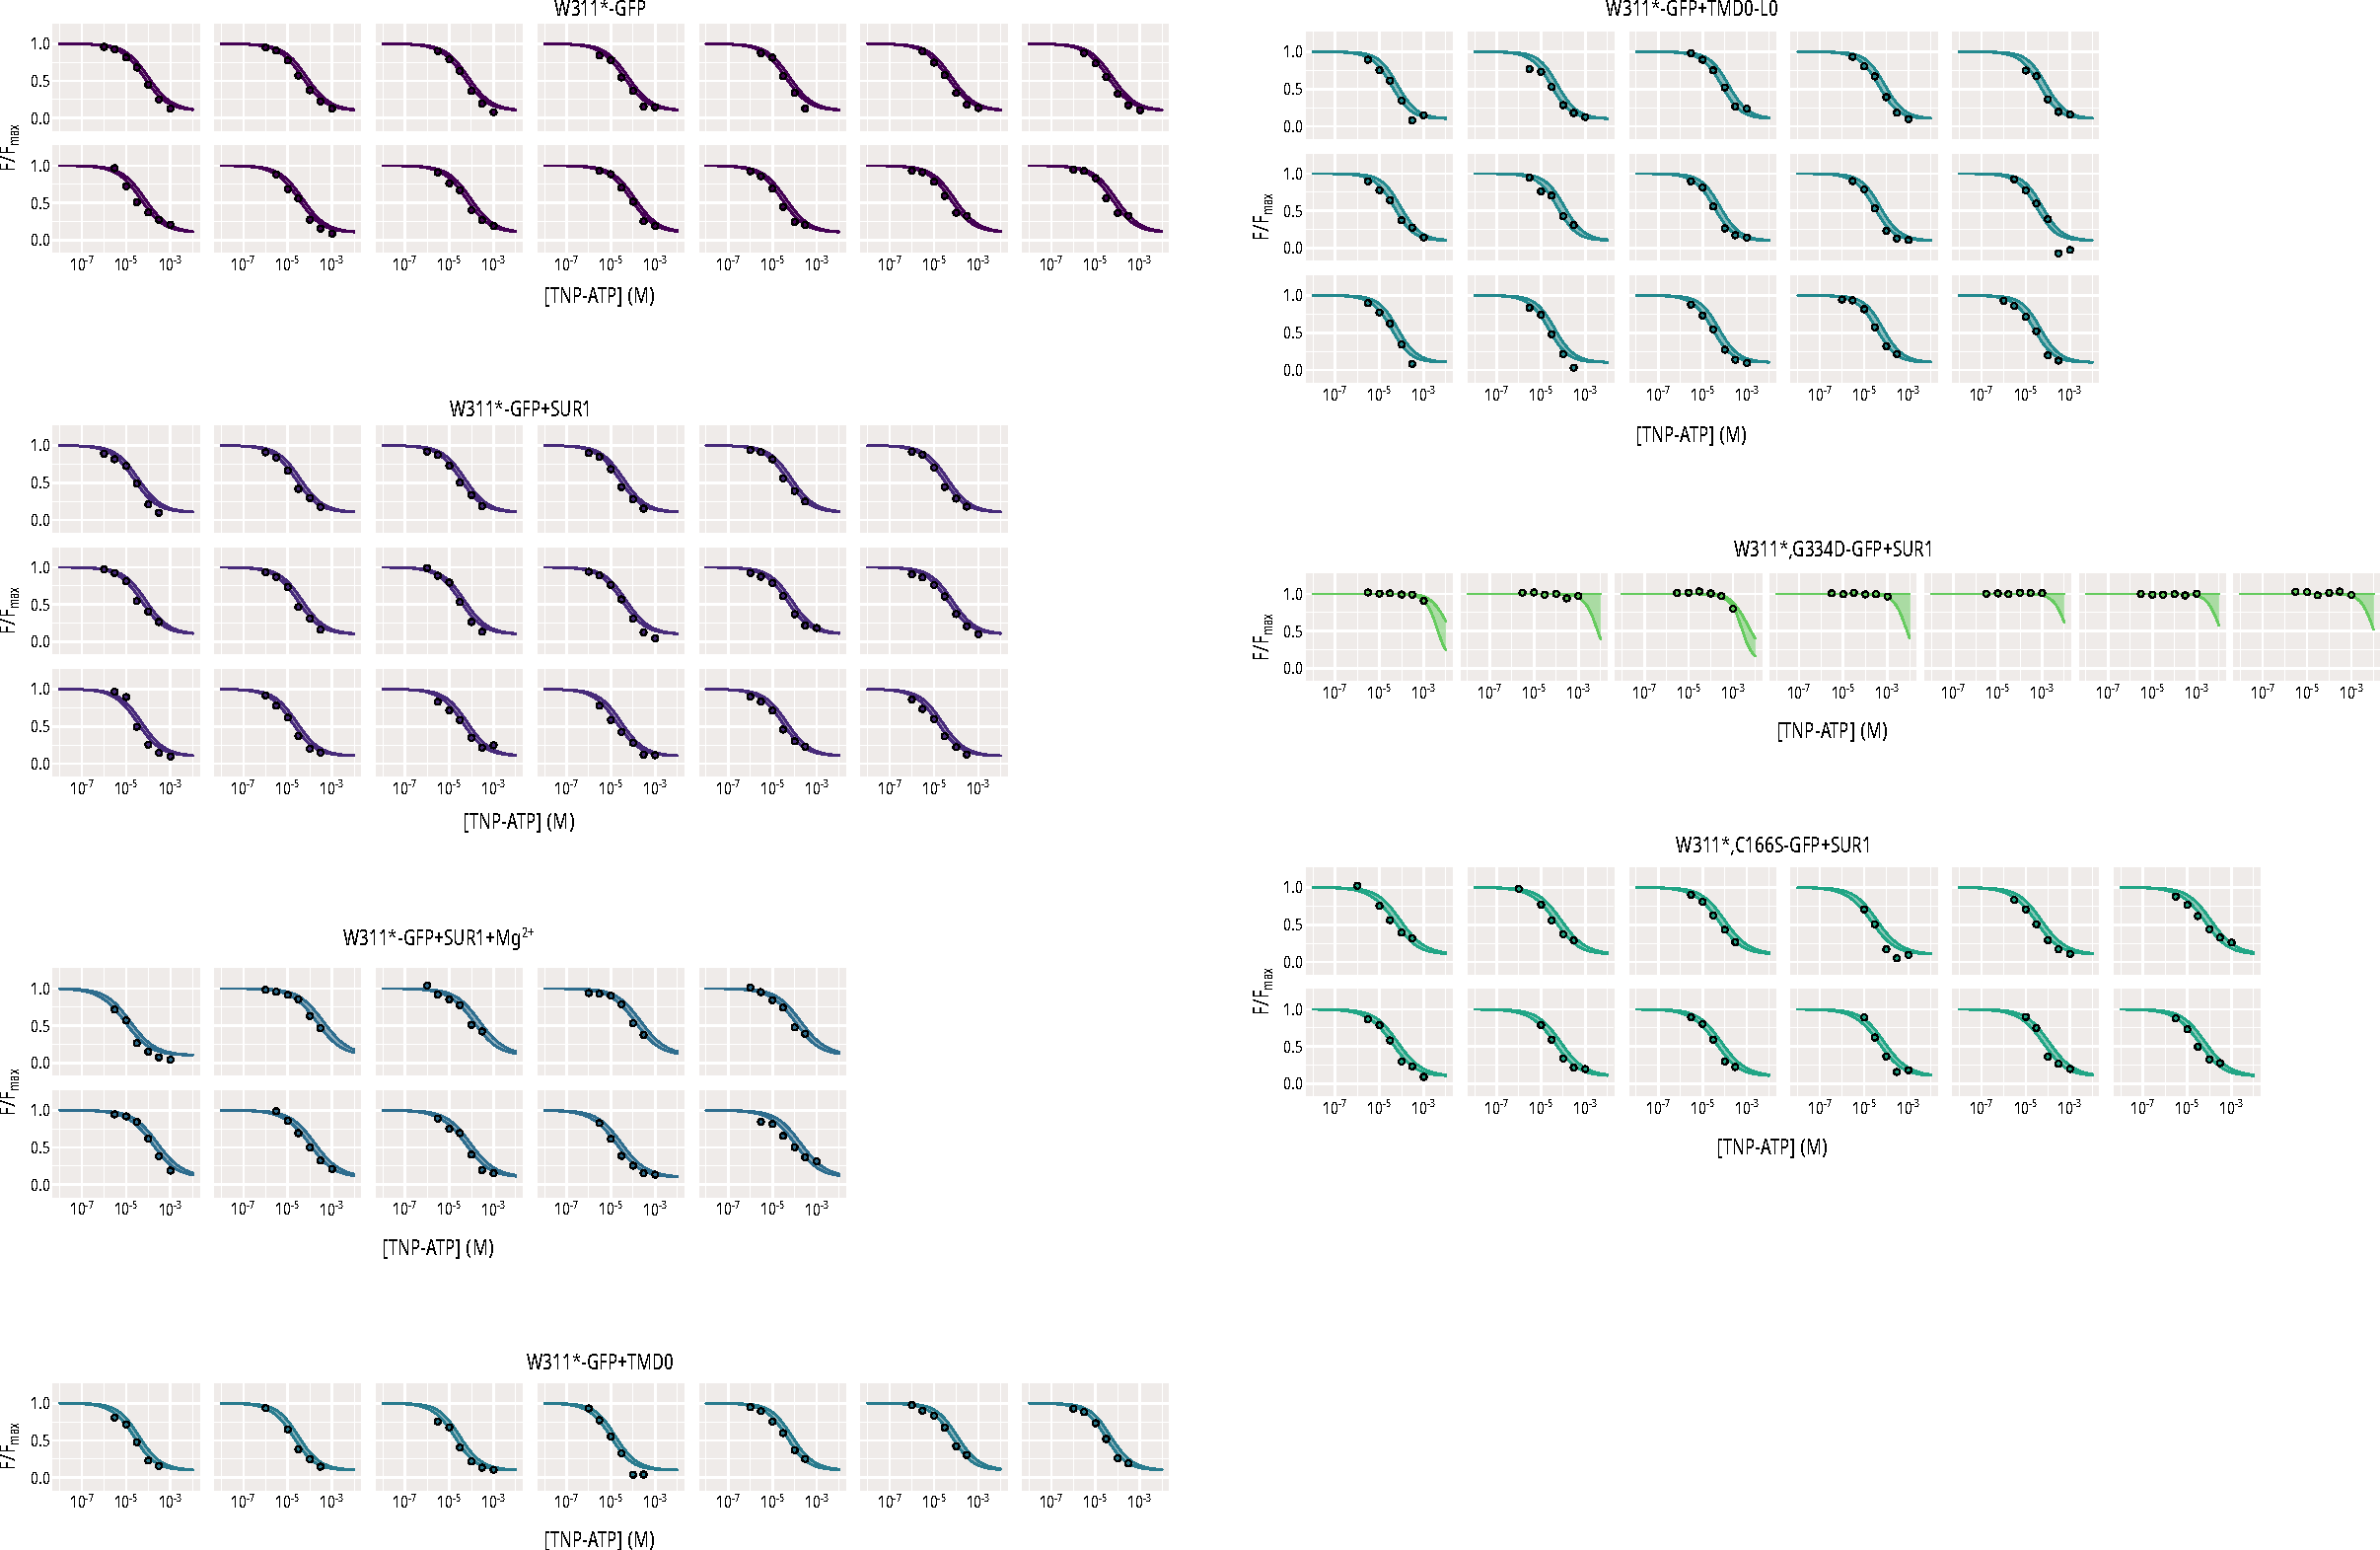
\includegraphics[width=\textwidth]{all_unroofed_fits_2.pdf}
	\caption[Unroofed membrane quenching sample hill fits]{
	Quenching of ANAP fluorescence by TNP-ATP in unroofed membrane patches expressing each of the constructs and conditions tested in this thesis, with each individual experiment plotted separately.
	Each point represents an individual measurement normalised to the average of the current measured immediately before TNP-ATP perfusion, and immediately after TNP-ATP washout.
	The smooth filled curves are the \SI{95}{\percent} intervals of the posterior probability distribution of fits to equation \ref{eq:hill} as described in the methods, including the \textgreek{d}\textsubscript{experiment}.
	}
	\label{apxfig:unroofed_2}
\end{figure}

\begin{figure}[h]
	\centering
	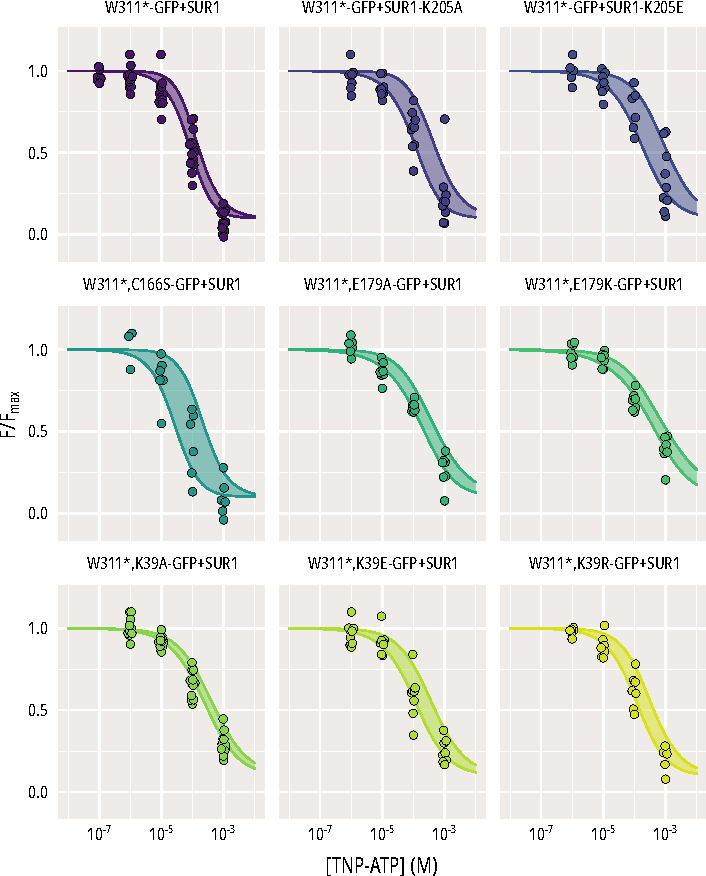
\includegraphics[width=\textwidth]{all_pcf_fits_3.pdf}
	\caption[Excised patch quenching population hill fits]{
	Quenching of ANAP fluorescence by TNP-ATP in excised patches expressing each of the constructs and conditions tested in this thesis.
	Each point represents an individual measurement normalised to the average of the current measured immediately before TNP-ATP perfusion, and immediately after TNP-ATP washout.
	The smooth filled curves are the \SI{95}{\percent} intervals of the posterior probability distribution of fits to equation \ref{eq:hill} as described in the methods, marginalising over the \textgreek{d}\textsubscript{experiment}.
	}
	\label{apxfig:pcf_1}
\end{figure}

\begin{figure}[h]
	\centering
	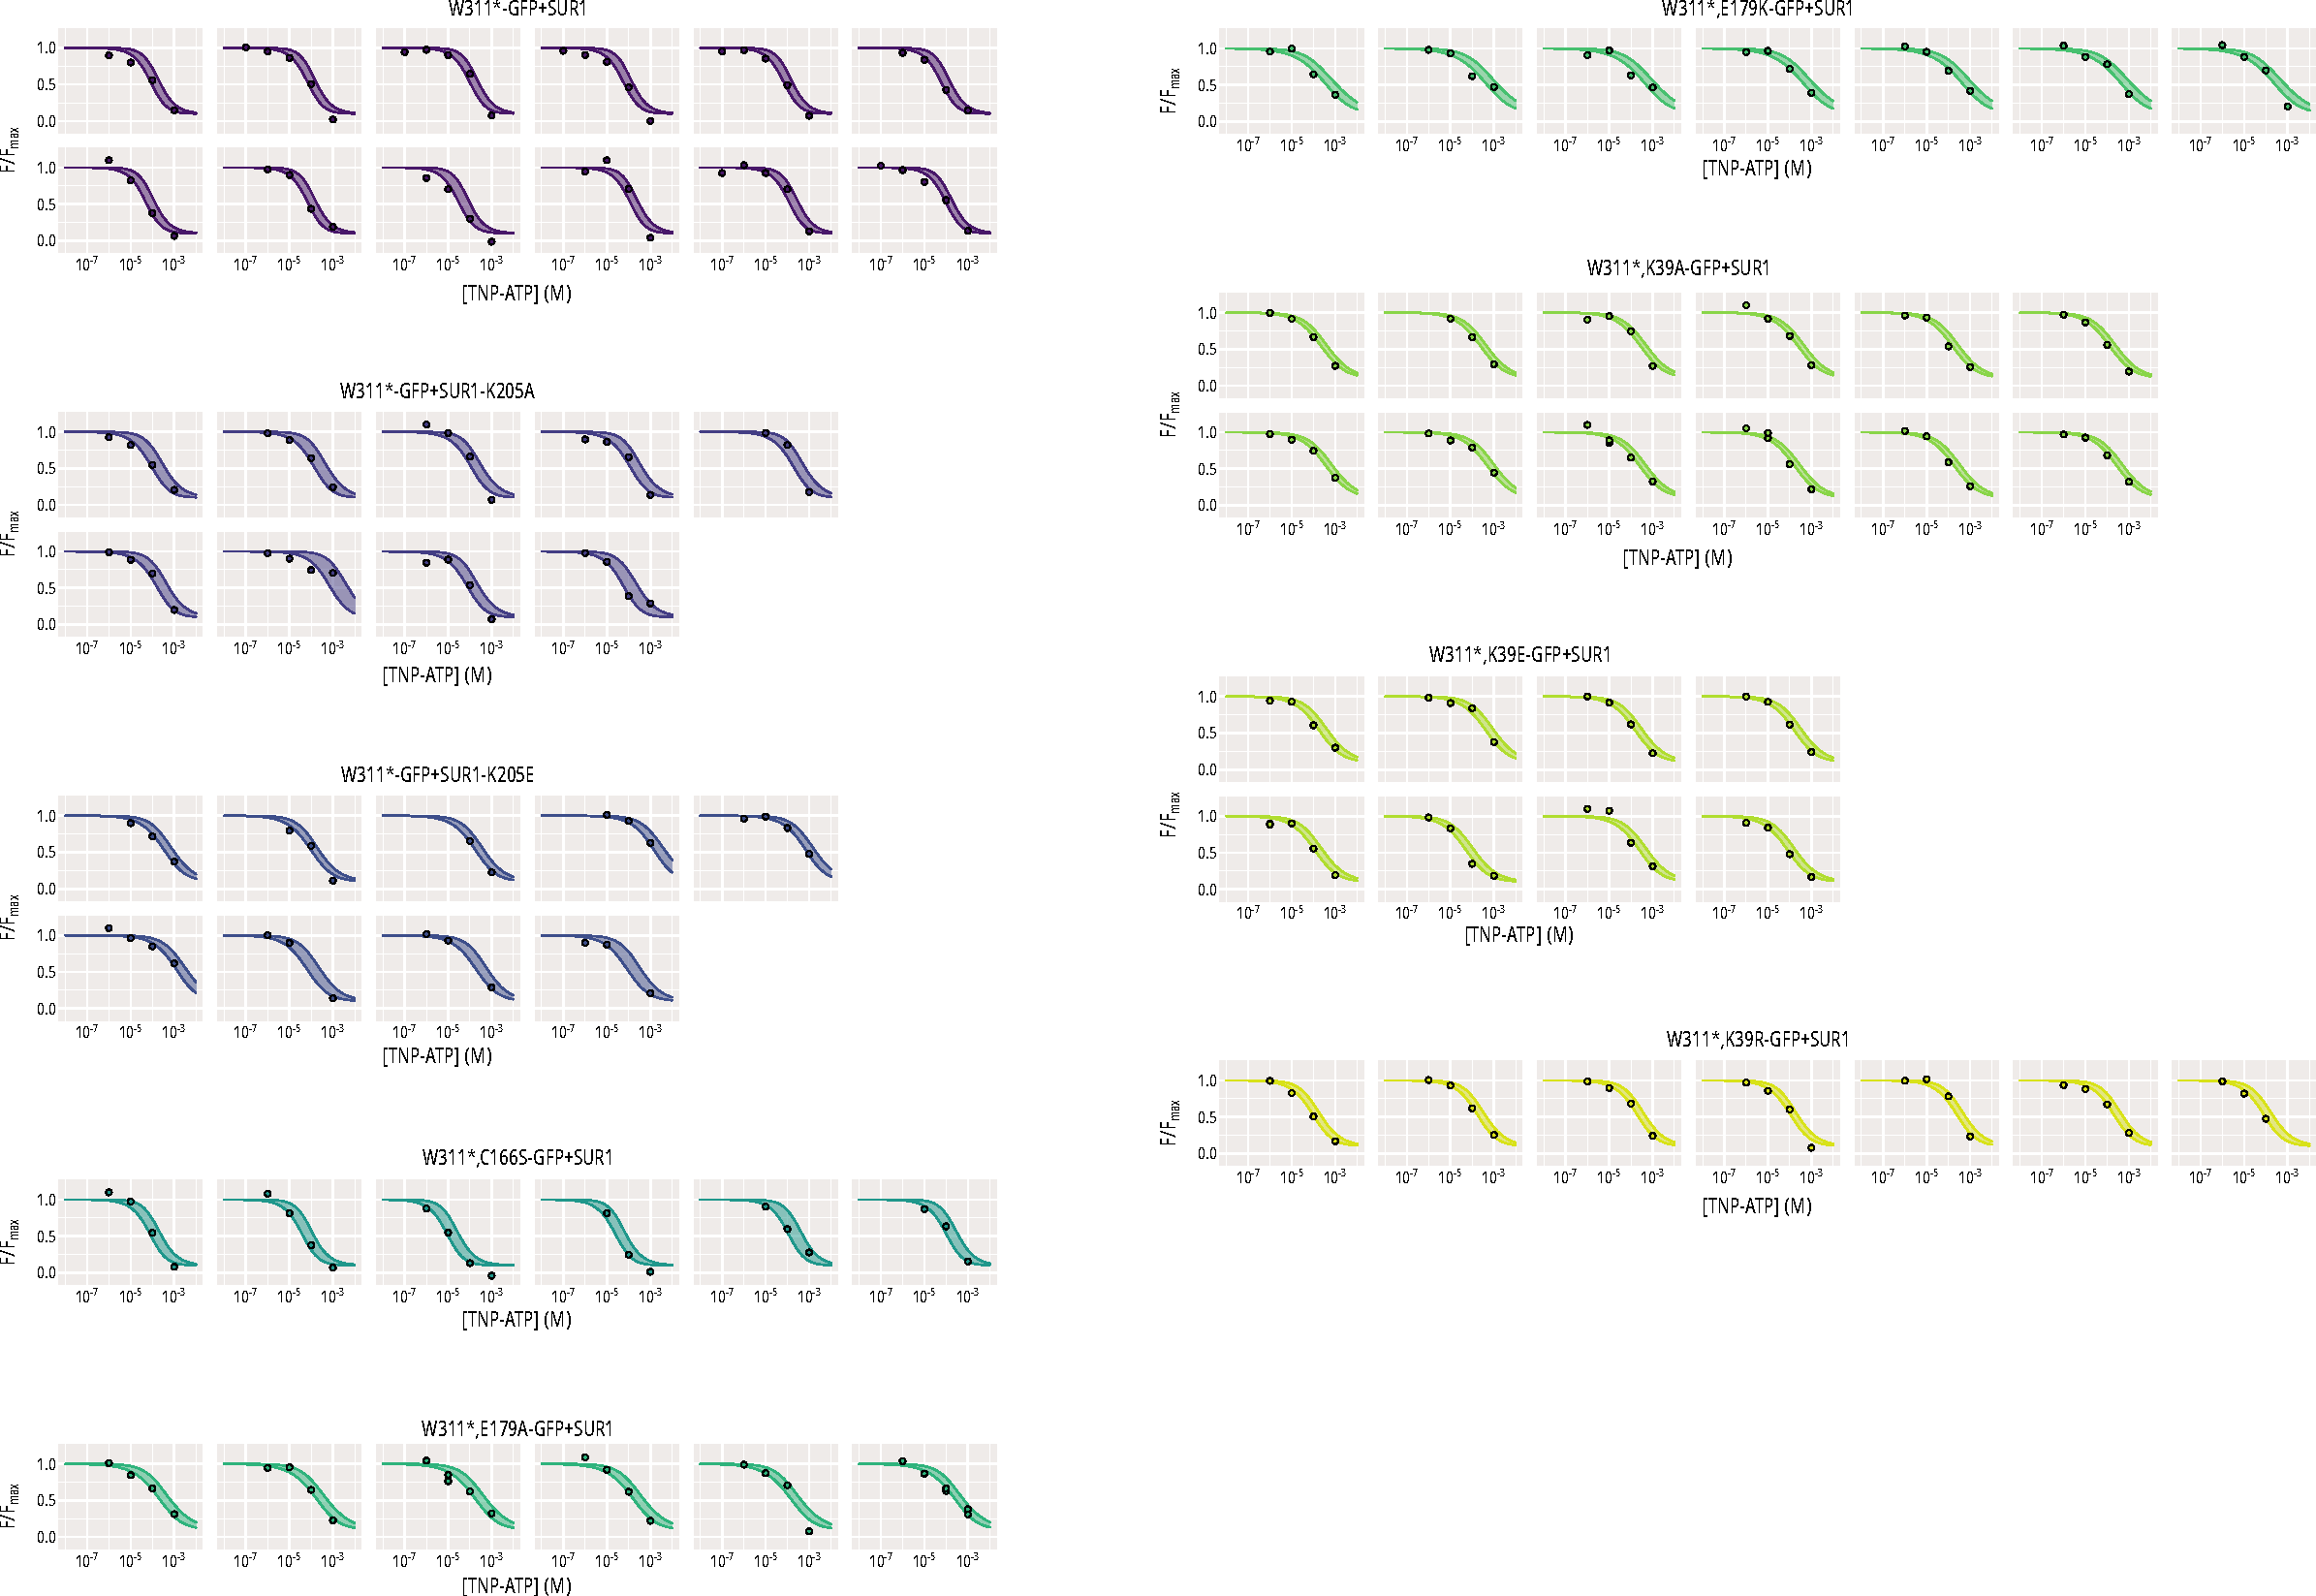
\includegraphics[width=\textwidth]{all_pcf_fits_4.pdf}
	\caption[Excised patch quenching sample hill fits]{
	Quenching of ANAP fluorescence by TNP-ATP in excised patches expressing each of the constructs and conditions tested in this thesis, with each individual experiment plotted separately.
	Each point represents an individual measurement normalised to the average of the current measured immediately before TNP-ATP perfusion, and immediately after TNP-ATP washout.
	The smooth filled curves are the \SI{95}{\percent} intervals of the posterior probability distribution of fits to equation \ref{eq:hill} as described in the methods, including the \textgreek{d}\textsubscript{experiment}.
	}
	\label{apxfig:pcf_2}
\end{figure}

\begin{figure}[h]
	\centering
	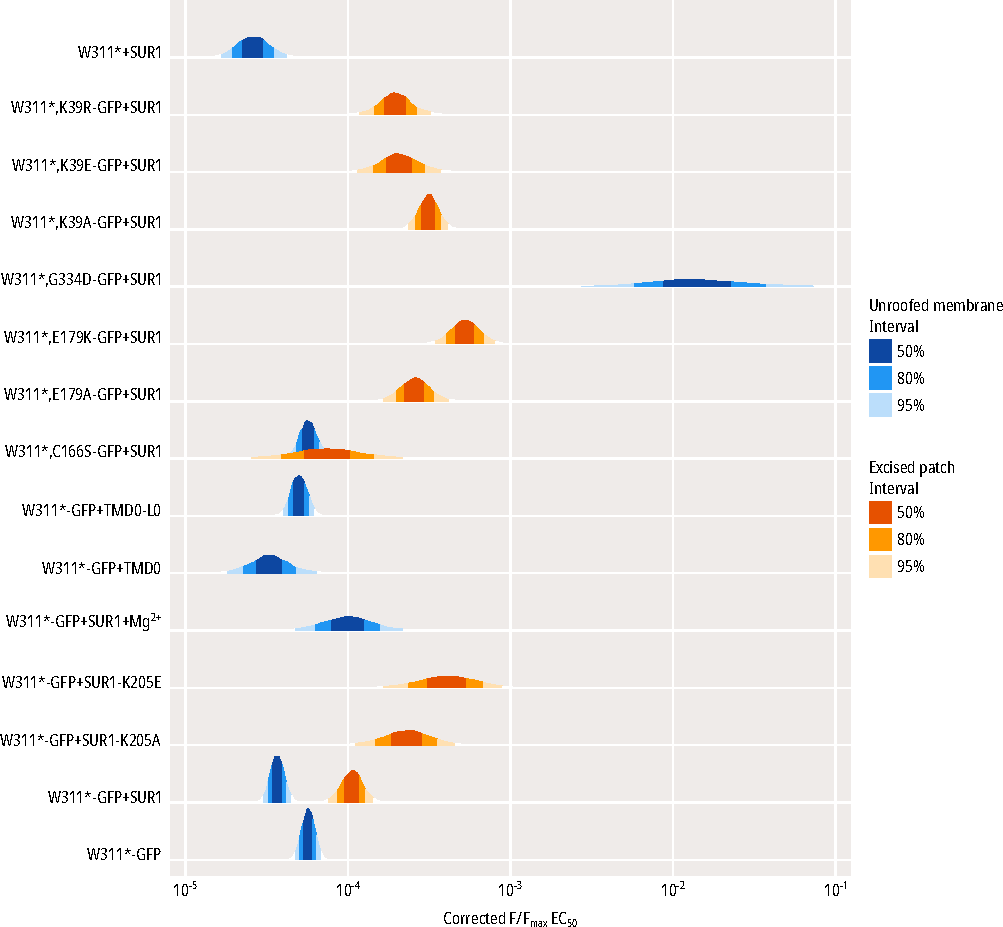
\includegraphics[width=\textwidth]{all_binding_params.pdf}
	\caption[Fluorescence quenching EC\textsubscript{50} posterior distributions]{
	Posterior probability distributions for the population $EC_{50}$ values for quenching by TNP-ATP in unroofed membrane patches (blue) or excised patches (orange) from the fits in Figures \ref{apxfig:unroofed_1} and \ref{apxfig:pcf_1}.
	}
	\label{apxfig:binding_params}
\end{figure}

\begin{figure}[h]
	\centering
	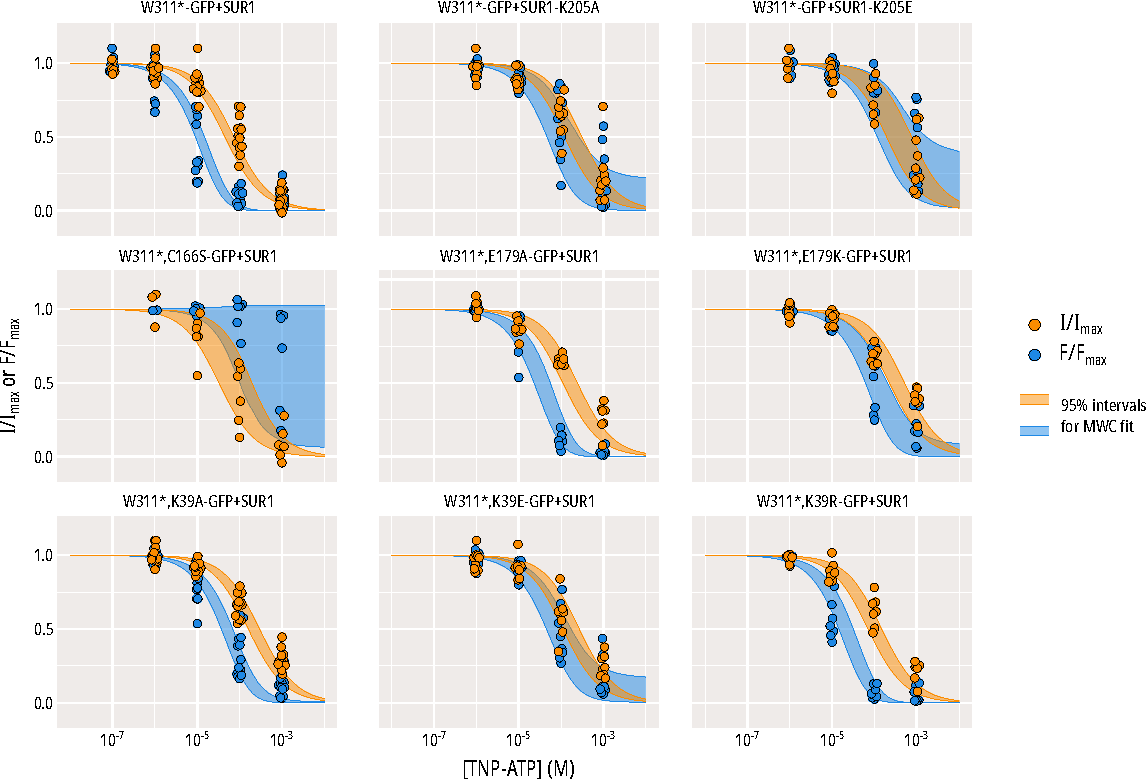
\includegraphics[width=\textwidth]{all_pcf_fits_1.pdf}
	\caption[MWC population fits]{
	Current inhibition (orange) and fluorescence quenching (blue) by TNP-ATP of all constructs tested in excised patches, data the same as Figure \ref{apxfig:tnpatp_inhib_1} and \ref{apxfig:pcf_1}.
	Fitted curves are the \SI{95}{\percent} intervals of the posterior probability distribution of fits to the MWC model paramaterised in equations \ref{eq:mwc_binding} and \ref{eq:normalised_po}, marginalising over the $\delta_{experiment}$
	}
	\label{apxfig:pcf_3}
\end{figure}

\begin{figure}[h]
	\centering
	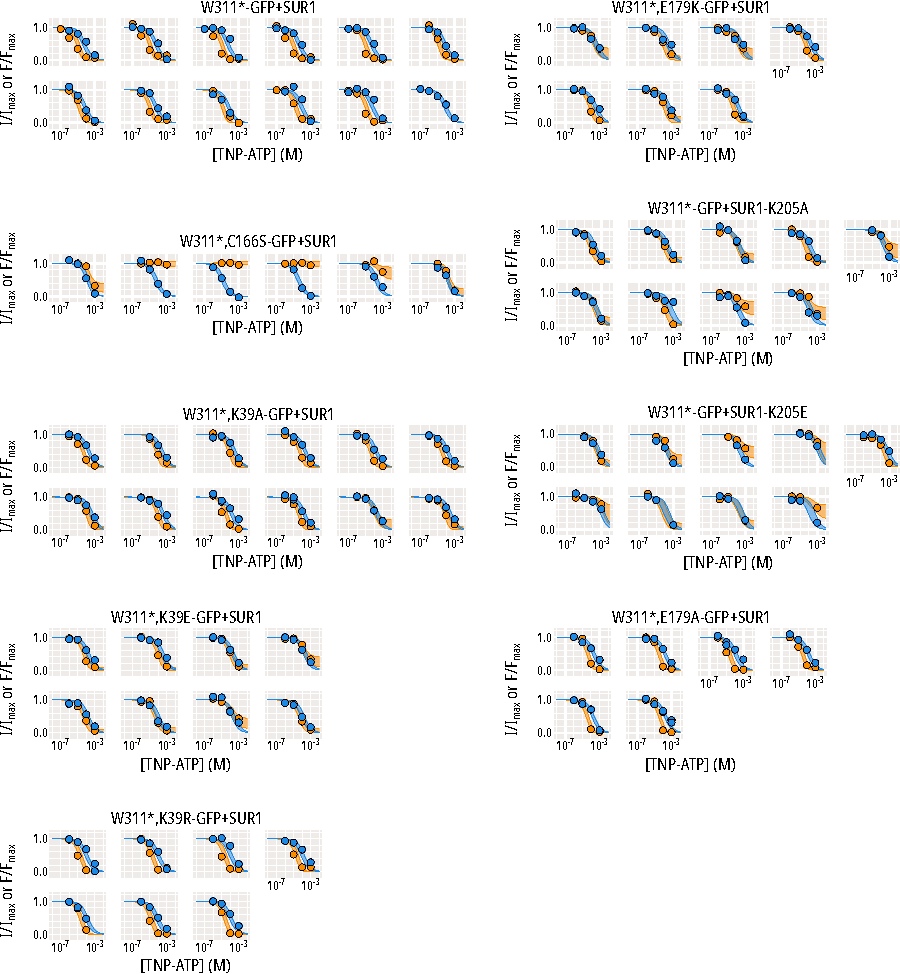
\includegraphics[width=\textwidth]{all_pcf_fits_2.pdf}
	\caption[MWC sample fits]{
	Current inhibition (orange) and fluorescence quenching (blue) by TNP-ATP of all constructs tested in excised patches with each individual experiment plotted separately, data the same as Figures \ref{apxfig:tnpatp_inhib_2} and \ref{apxfig:pcf_2}.
	Fitted curves are the \SI{95}{\percent} intervals of the posterior probability distribution of fits to the MWC model paramaterised in equations \ref{eq:mwc_binding} and \ref{eq:normalised_po}, including the $\delta_{experiment}$
	}
	\label{apxfig:pcf_4}
\end{figure}

\begin{figure}[h]
	\centering
	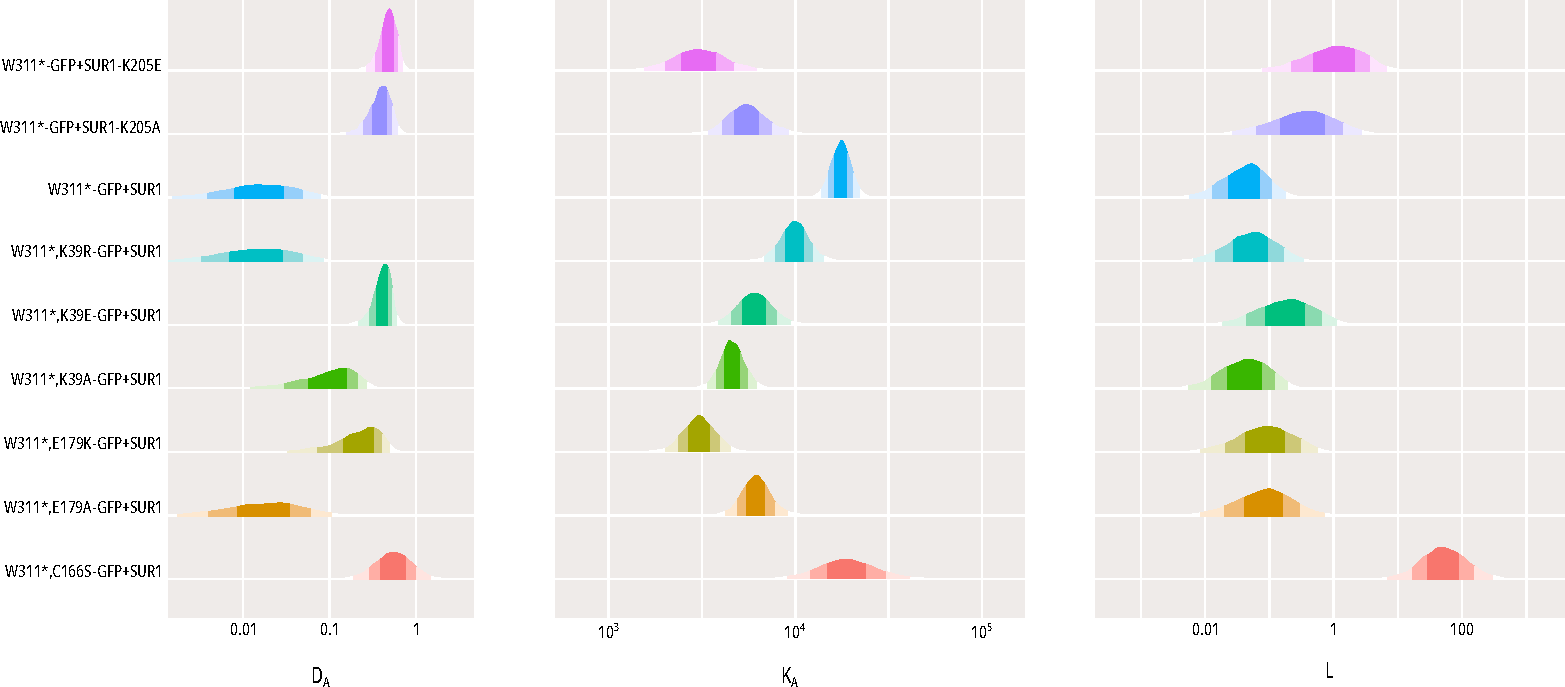
\includegraphics[width=\textwidth,angle=90,origin=c]{all_pcf_params_1.pdf}
	\caption[MWC parameter posterior distributions]{
	Posterior probability distributions for the population parameter values from equations \ref{eq:mwc_binding} and \ref{eq:normalised_po} for the MWC fits in Figure \ref{apxfig:pcf_3}.
	}
	\label{apxfig:mwc_params}
\end{figure}

\begin{figure}[h]
	\begin{subfigure}[t]{0.3\textwidth}
		\caption{}\label{apxfig:inhib_cc_1}
		\centering
		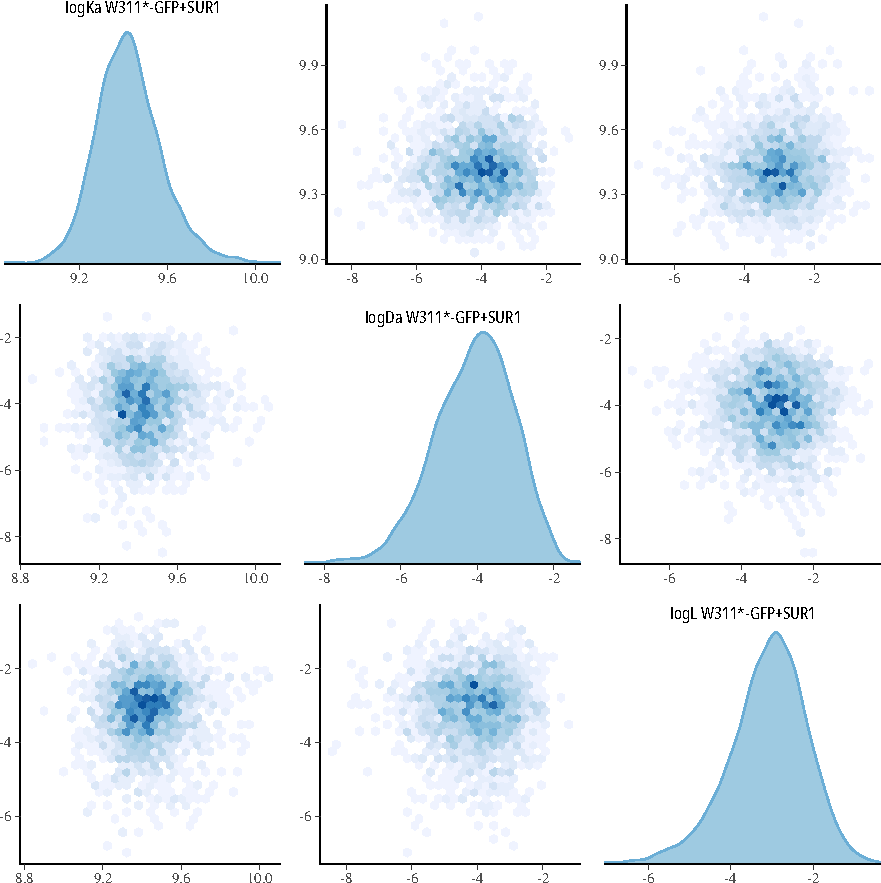
\includegraphics[width=\textwidth]{inhibition_crosscorr_1.pdf}
	\end{subfigure}
	\hfill
	\begin{subfigure}[t]{0.3\textwidth}
		\caption{}\label{apxfig:inhib_cc_2}
		\centering
		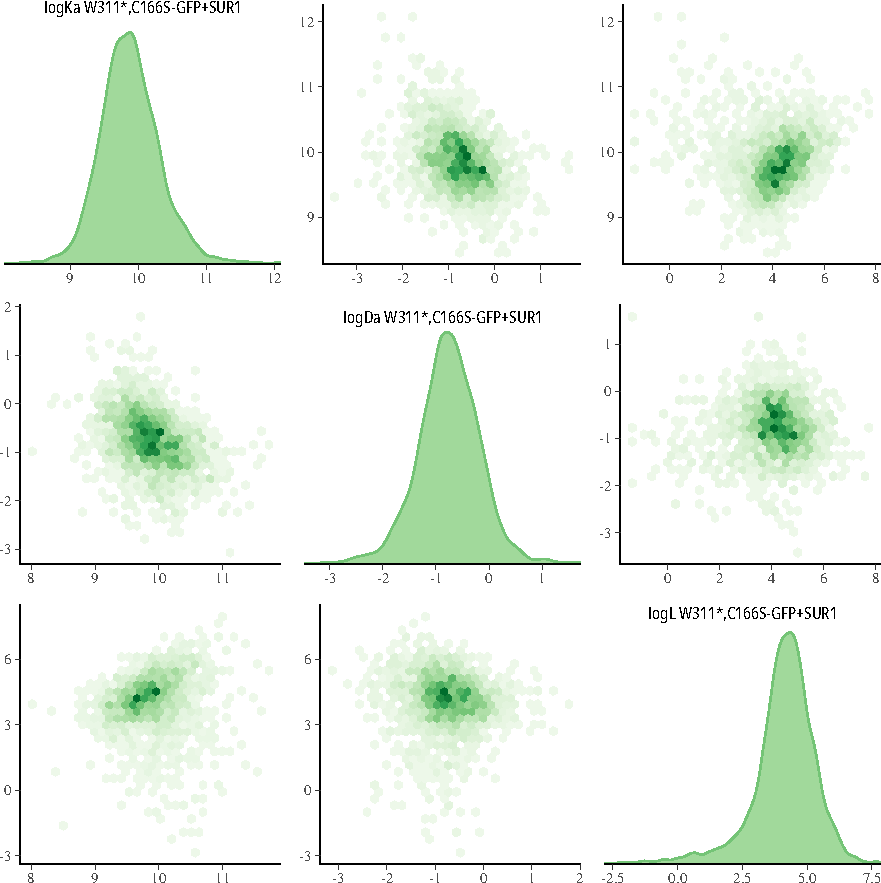
\includegraphics[width=\textwidth]{inhibition_crosscorr_2.pdf}
	\end{subfigure}
	\hfill
	\begin{subfigure}[t]{0.3\textwidth}
		\caption{}\label{apxfig:inhib_cc_3}
		\centering
		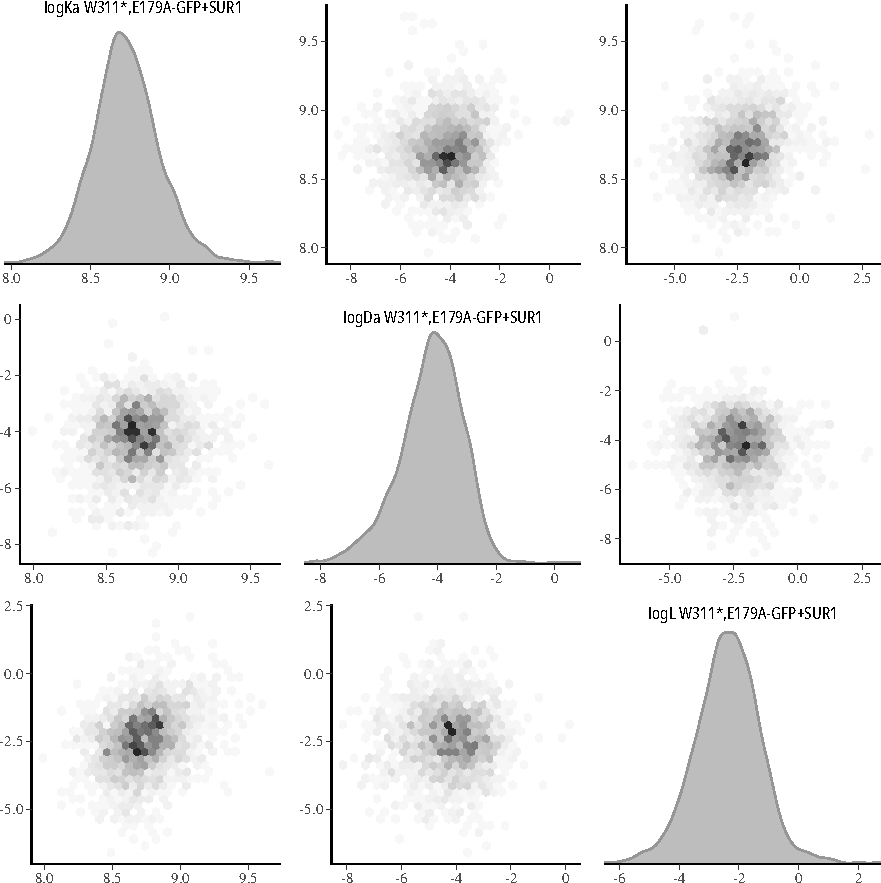
\includegraphics[width=\textwidth]{inhibition_crosscorr_3.pdf}
	\end{subfigure}
	\vfill
	\begin{subfigure}[t]{0.3\textwidth}
		\caption{}\label{apxfig:inhib_cc_4}
		\centering
		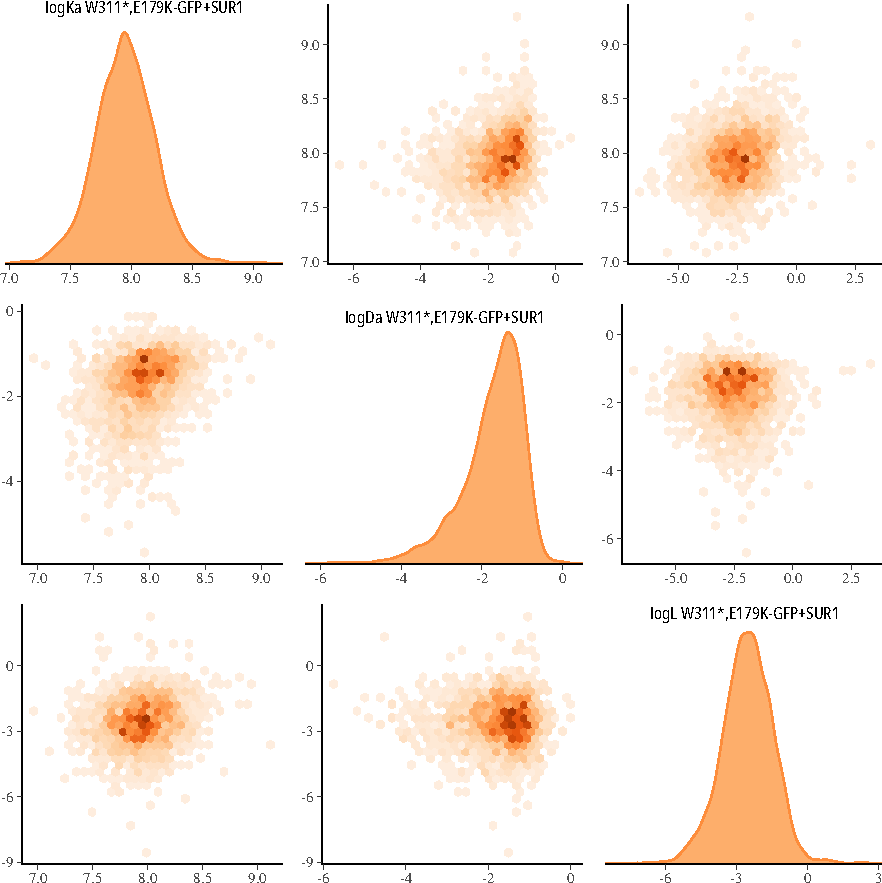
\includegraphics[width=\textwidth]{inhibition_crosscorr_4.pdf}
	\end{subfigure}
	\hfill
	\begin{subfigure}[t]{0.3\textwidth}
		\caption{}\label{apxfig:inhib_cc_5}
		\centering
		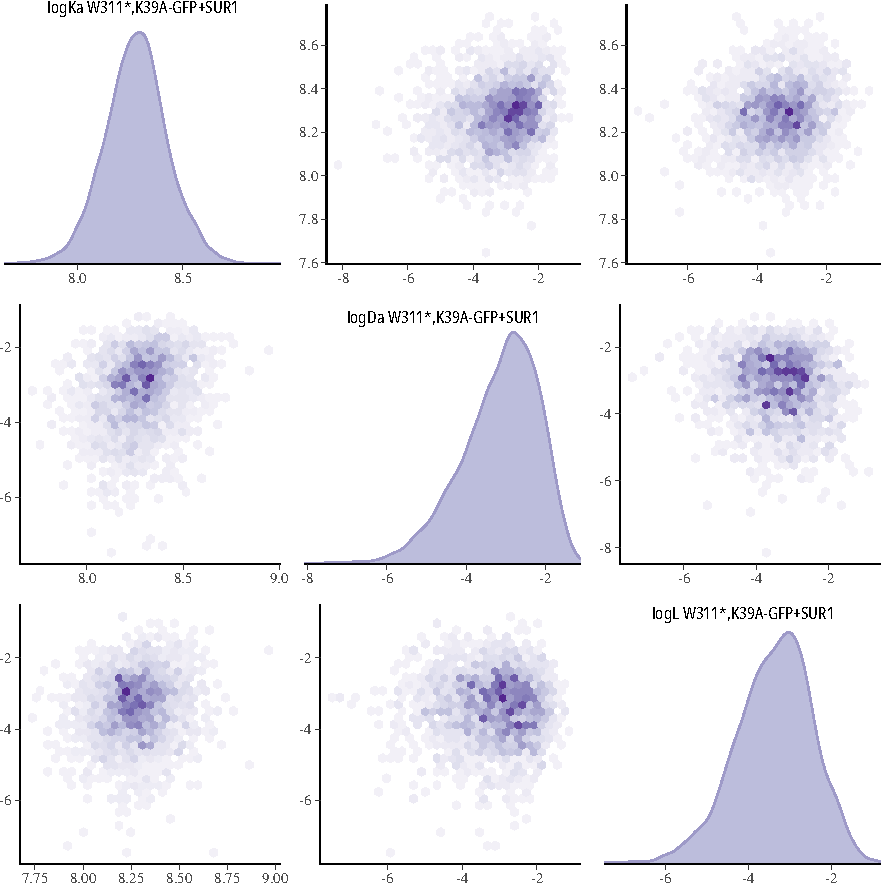
\includegraphics[width=\textwidth]{inhibition_crosscorr_5.pdf}
	\end{subfigure}
	\hfill
	\begin{subfigure}[t]{0.3\textwidth}
		\caption{}\label{apxfig:inhib_cc_6}
		\centering
		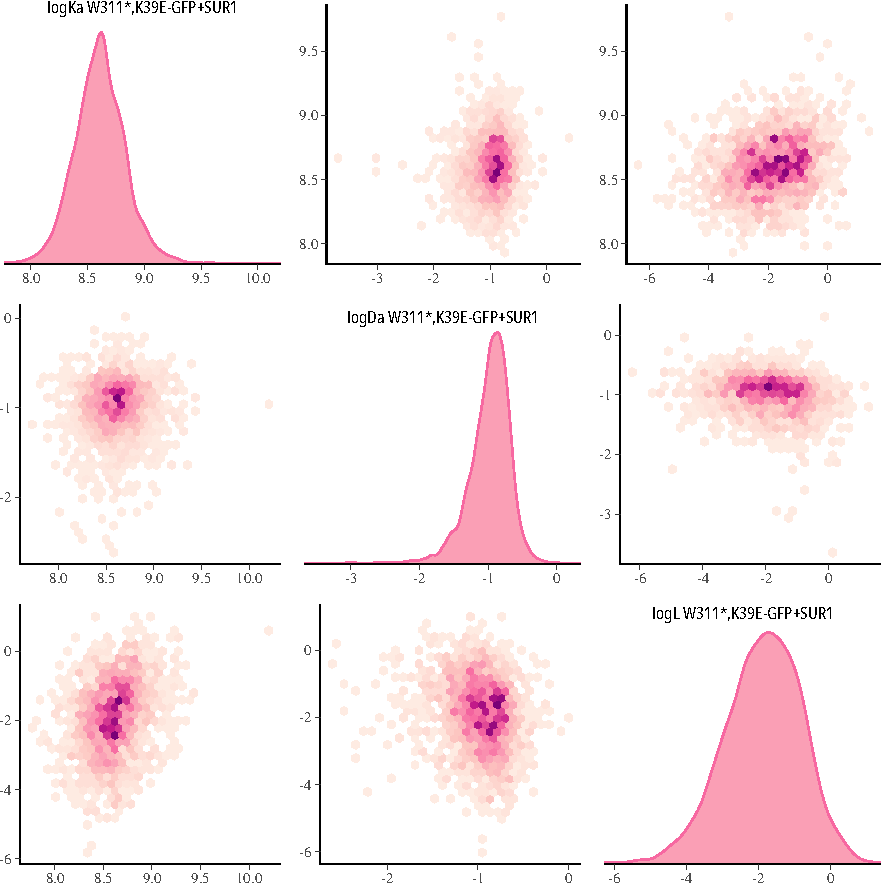
\includegraphics[width=\textwidth]{inhibition_crosscorr_6.pdf}
	\end{subfigure}
	\vfill
	\begin{subfigure}[t]{0.3\textwidth}
		\caption{}\label{apxfig:inhib_cc_7}
		\centering
		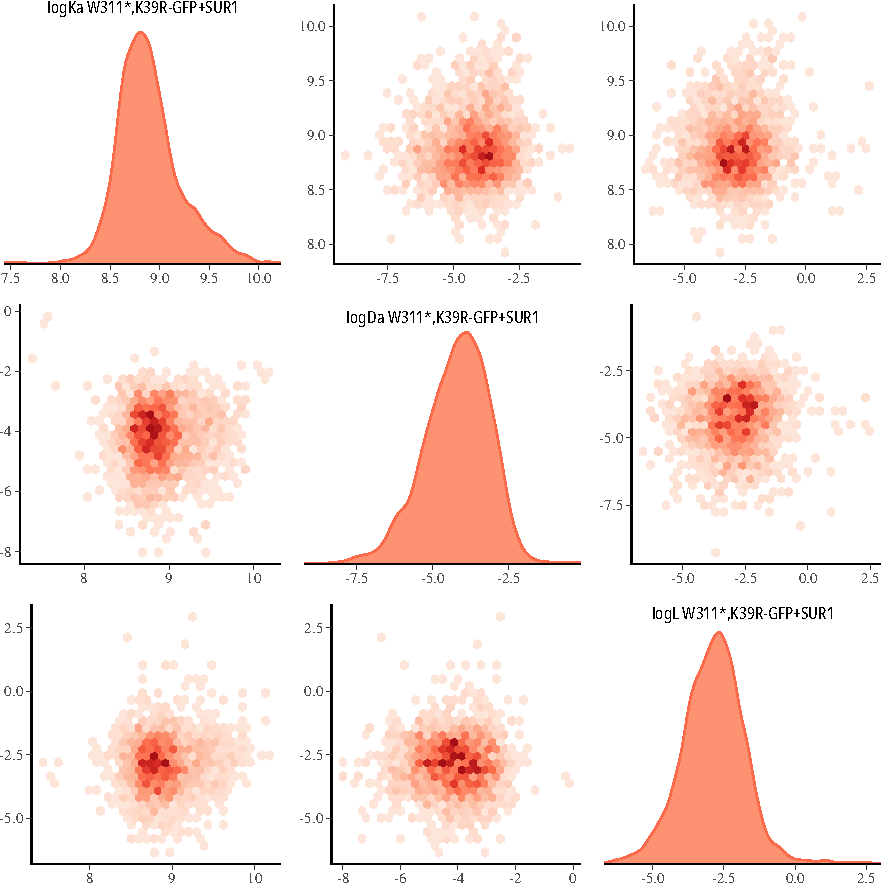
\includegraphics[width=\textwidth]{inhibition_crosscorr_7.pdf}
	\end{subfigure}
	\hfill
	\begin{subfigure}[t]{0.3\textwidth}
		\caption{}\label{apxfig:inhib_cc_8}
		\centering
		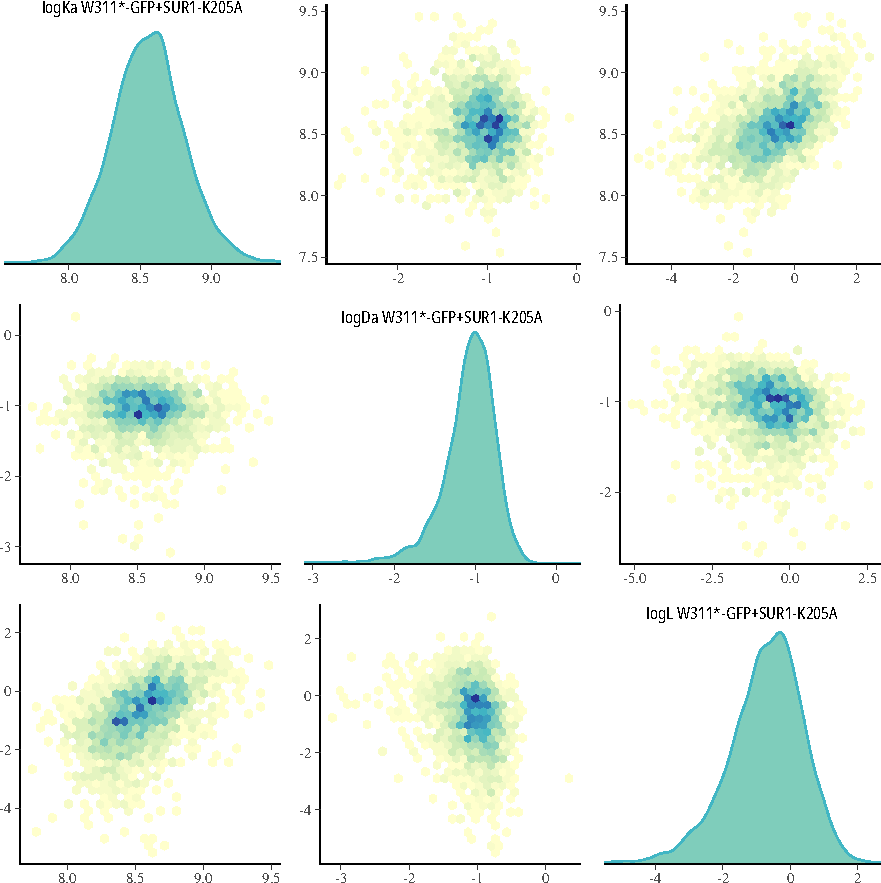
\includegraphics[width=\textwidth]{inhibition_crosscorr_8.pdf}
	\end{subfigure}
	\hfill
	\begin{subfigure}[t]{0.3\textwidth}
		\caption{}\label{apxfig:inhib_cc_9}
		\centering
		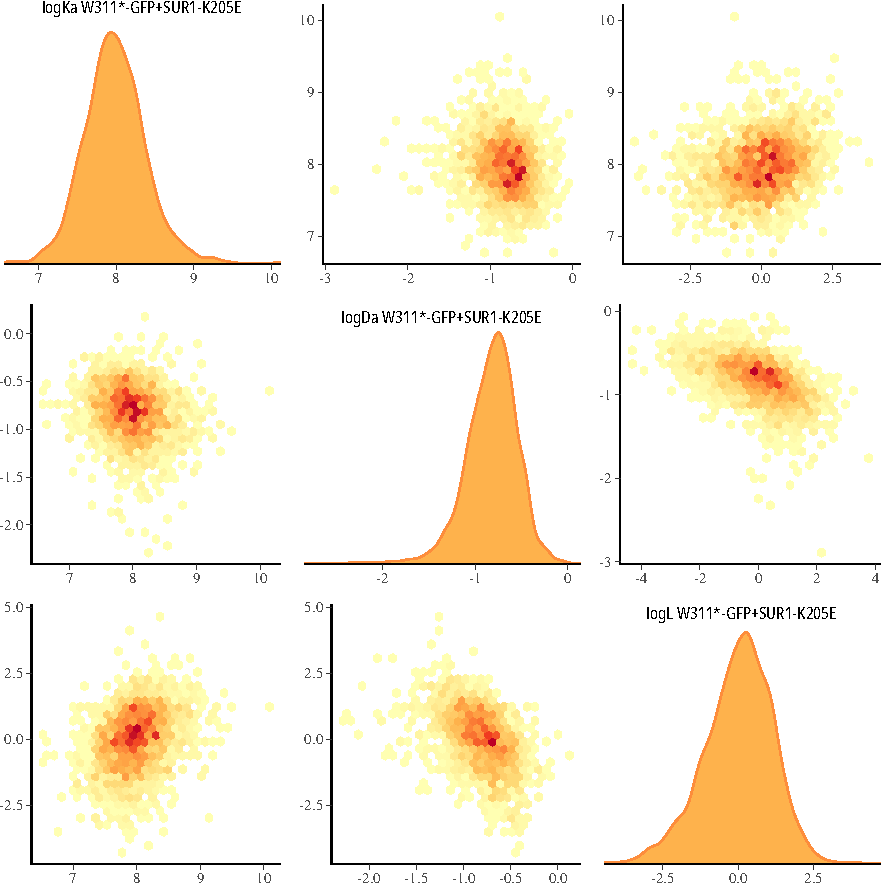
\includegraphics[width=\textwidth]{inhibition_crosscorr_9.pdf}
	\end{subfigure}
	\caption[MWC parameter cross-correlation - inhibition]{
	Cross correlation plots of the parameter estimates of the MWC model paramaterised in equations \ref{eq:mwc_binding} and \ref{eq:normalised_po} for each construct tested.
	}
	\label{apxfig:inhibition_crosscorr}
\end{figure}

\begin{figure}[h]
	\centering
	\includegraphics[width=\textwidth]{activation_crosscorr_1.pdf}
	\caption[MWC parameter cross-correlation - inhibition and activation]{
	Cross correlation plots of the parameter estimates of the MWC model including the inhibition data collected in this thesis and the activation data from reference \cite{puljung_activation_2019-1}
	}
	\label{apxfig:activation_crosscorr}
\end{figure}